\scanpage{25}
\noindent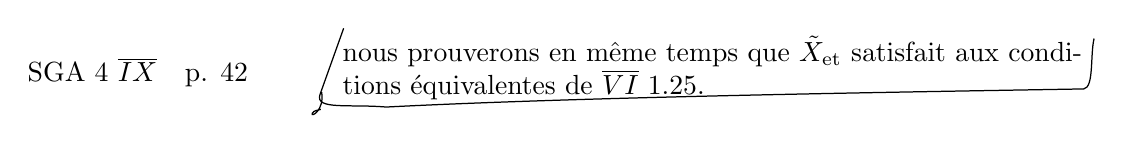
\begin{tikzpicture}[x=1cm,y=1cm]
\node[anchor=west,inner sep=0pt] at (0,-.35) {\handwritten{SGA 4 $\overline{\text{\uline{IX}}}$\quad p. 42}};
\node[anchor=north west,inner sep=0pt,text width=9.4cm] at (4.0,.12) {\handwritten{nous prouverons en même temps que $\tilde{X}_{\mathrm{et}}$ satisfait aux conditions équivalentes de $\overline{\text{\uline{VI}}}$ 1.25.}};
\draw[line width=.45pt] (4.02,.21) -- (3.72,-.63) .. controls (3.65,-.83) and (4.08,-.75) .. (4.56,-.79) .. controls (7.1,-.66) and (11.1,-.60) .. (13.42,-.56) .. controls (13.55,-.54) and (13.50,-.13) .. (13.55,.08);
\draw[line width=.45pt] (3.74,-.60) .. controls (3.78,-.83) and (3.60,-.93) .. (3.62,-.87) .. controls (3.64,-.83) and (3.70,-.83) .. (3.73,-.82);
\end{tikzpicture}

\handwritten{(*) (Note pour la page 8.) Prouvons que la notion de constructibilité 2.3 pour un faisceau d'ensembles $F$ coïncide avec celle de $\overline{\text{\uline{VI}}}$ 1.9.3. \deleted{Soit} La \deleted{en effet $C$ le \unsure{cas}}\inserted{question étant} locale sur $X$, on peut supposer $X$ affine \inserted{donc ``cohérent'', i.e.} quasi-compact et quasi-séparé. \deleted{Soit $C$ la catégorie \unsure{Soit $(C')$ le sous}\illegible{1}} \deleted{Je faut alors prouver que $F$ est constructible} Soit $C$ (resp. $C'$) la sous-catégorie \deleted{\unsure{pleine}}\inserted{strictement} pleine de $\tilde{X}_{\mathrm{et}}$ formée des $F$ constructibles au sens de 2.3, \deleted{\illegible{1}} \inserted{(resp. au sens de $\overline{\text{\uline{VI}}}$ 1.9.3), il} faut prouver \deleted{que $C$ s'identifie à la catégorie des objets \uline{cohérents} de} \deleted{$\tilde{X}_{\mathrm{et}}$} que $C=C'$;}

\reversemarginpar
\margin{\handwritten{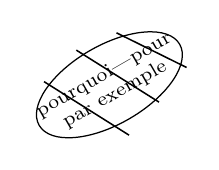
\begin{tikzpicture}[x=1cm,y=1cm]
\node[rotate=30,align=center,inner sep=0pt,font=\scriptsize] at (0,0) {\unsure{pourquoi|pour}\\\unsure{par exemple}};
\draw[line width=.45pt,rotate=30] (0,0) ellipse[x radius=1.03,y radius=.50];
\draw[line width=.55pt] (-.83,.04)--(.25,-.64);
\draw[line width=.55pt] (-.42,.44)--(.63,-.22);
\draw[line width=.55pt] (.09,.66)--(.98,.22);
\end{tikzpicture}}}
\normalmarginpar

% Entire argument cancelled by the enclosing irregular strokes and long obliques.
% Coordinates below reproduce the source geometry relative to (230,470).
\figure{\begin{tikzpicture}[x=.0085cm,y=-.0085cm]
\node[anchor=base west,inner sep=0pt,rotate=4,font=\scriptsize] at (345,80) {\handwritten{En vertu de $\overline{\text{\uline{VII}}}$ 5.6 a), \deleted{l'objet final $X$ de} $\tilde{X}_{\mathrm{et}}$}};
\node[anchor=base west,inner sep=0pt,rotate=4,font=\scriptsize] at (0,184) {\handwritten{\deleted{est cohérent, donc} $C'$ est formé des objets \uline{cohérents} \deleted{\unsure{\uline{VI}}} de $\tilde{X}_{\mathrm{et}}$ (2.5).}};
\node[anchor=base west,inner sep=0pt,rotate=4,font=\scriptsize] at (0,235) {\handwritten{En vertu de $\overline{\text{\uline{VI}}}$ 1.24, \deleted{\unsure{et}} et compte tenu du fait que $C$ est génératrice}};
\node[anchor=base west,inner sep=0pt,rotate=4,font=\scriptsize] at (0,310) {\handwritten{dans $\tilde{X}_{\mathrm{et}}$ (2.7.2) et stable par limites inductives finies (2.\unsure{6|8} (i)),}};
\node[anchor=base west,inner sep=0pt,rotate=4,font=\scriptsize] at (0,365) {\handwritten{il suffit de prouver que $C\subset C'$, Mais il résulte de 2.7 que tout}};
\node[anchor=base west,inner sep=0pt,rotate=4,font=\scriptsize] at (0,430) {\handwritten{$F\in\mathrm{ob}\,C$ est \uline{quasi-compact}, puisque un \deleted{\unsure{$G\in\mathrm{ob}\,X_{\mathrm{et}}$}} \deleted{\unsure{représentable} par un}}};
\node[anchor=base west,inner sep=0pt,rotate=4,font=\scriptsize] at (932,321) {\handwritten{\inserted{$\unsure{G|C}\in\unsure{X'_{\mathrm{et}}|X_{\mathrm{ét}}}$}}};
\node[anchor=base west,inner sep=0pt,rotate=4,font=\scriptsize] at (0,503) {\handwritten{\deleted{schéma $\unsure{X'|X'_{\mathrm{et}}}$} qui est quasi-compact et quasi-séparé est quasi-compact}};
\node[anchor=base west,inner sep=0pt,rotate=4,font=\scriptsize] at (0,565) {\handwritten{comme objet de $\tilde{X}_{\mathrm{et}}$ \deleted{(5.6.1)} ($\overline{\text{\uline{VII}}}$ 5.6.1). \deleted{D'autre part pour}}};
\node[anchor=base west,inner sep=0pt,rotate=4,font=\scriptsize] at (0,625) {\handwritten{\deleted{voir que $\unsure{F|F'}\unsure{\in|\to}\unsure{\mathrm{ob}\,X'|X'}$ la diagonale $F\longrightarrow F\mathbin{\times}_{X}F$ est quasi-compacte,}}};
\node[anchor=base west,inner sep=0pt,rotate=4,font=\scriptsize] at (0,699) {\handwritten{\deleted{il suffit de voir que \unsure{pour tout} \illegible{2} \unsure{et que}\illegible{2}}}};
\node[anchor=base west,inner sep=0pt,rotate=4,font=\scriptsize] at (0,763) {\handwritten{\deleted{\unsure{ce fait que $C$ est stable par produits}} Comme $C$ est stable par \deleted{limites projectives}\inserted{produits}}};
\node[anchor=base west,inner sep=0pt,rotate=4,font=\scriptsize] at (0,820) {\handwritten{finis\inserted{(2.6 (ii))}, l'inclusion $C\subset C'$ est donc un cas particulier de 2.1.}};
% Irregular boundary, notched at the upper left, and the stepped cancellation line.
\draw[line width=.55pt] (318,20)--(318,145)--(8,179)--(22,818) .. controls (400,785) and (1020,735) .. (1360,692) .. controls (1405,684) and (1420,642) .. (1420,610);
\draw[line width=.55pt] (9,417)--(750,330)--(714,338)--(714,276)--(1369,231);
% Long oblique cancellation strokes.
\draw[line width=.60pt] (12,190)--(360,730);
\draw[line width=.60pt] (270,155)--(650,740);
\draw[line width=.60pt] (390,20)--(900,735);
\draw[line width=.60pt] (705,18)--(1145,705);
\draw[line width=.60pt] (917,-7)--(1365,645);
\draw[line width=.60pt] (1190,-20)--(1416,328);
\draw[line width=.50pt] (1325,-36)--(1415,66);
% Nested, stepped enclosure and cross-hatching over the abandoned diagonal test.
\draw[line width=.60pt] (918,458)--(1370,418)--(1385,478);
\draw[line width=.60pt] (1385,478) .. controls (1390,520) and (1390,548) .. (1370,548)--(725,610)--(477,643)--(477,723)--(0,762)--(-8,696)--(0,610)--(918,511);
\draw[line width=.50pt] (0,610)--(1380,501);
\draw[line width=.50pt] (-8,696)--(725,610);
\foreach \x in {935,1010,1085,1160,1235,1310}{\draw[line width=.55pt] (\x,450)--(\x+62,521);\draw[line width=.55pt] (\x+13,521)--(\x+68,443);}
\foreach \x in {0,75,150,225,300,375,450,525,600}{\draw[line width=.55pt] (\x,610)--(\x+53,691);\draw[line width=.55pt] (\x+9,693)--(\x+62,610);}
\draw[line width=.55pt] (77,749)--(380,673);
\draw[line width=.55pt] (205,743)--(430,661);
\end{tikzpicture}}

\handwritten{En vertu de $\overline{\text{\uline{VI}}}$ 2.9, b), il suffit de voir que $C$ est stable pour limites inductives finies et limites projectives finies, qu'elle est génératrice, et formée d'objets quasi-compacts. \deleted{\illegible{1}} Compte tenu de 2.6 (i) et (2.7.2), il reste à prouver que tout $F\in\mathrm{ob}\,C$ est quasi-compact. Or \deleted{cela résulte}\inserted{en vertu} de 2.7 \deleted{et $\overline{\text{\uline{VI}}}$ 1.3}, \deleted{puisque}\inserted{il existe} un $G\in\mathrm{ob}\,X_{\mathrm{et}}$ \deleted{\illegible{1}} qui est \inserted{un schéma} quasi-compact et quasi-séparé \deleted{\unsure{et est}} et un épimorphisme $G\longrightarrow F$. Or $G$ \deleted{\unsure{comme on}} est un objet quasi-compact de $\tilde{X}_{\mathrm{et}}$ ($\overline{\text{\uline{VII}}}$ 5.6.1), donc $F$ est quasi-compact ($\overline{\text{\uline{VI}}}$ 1.3), qfd.}

\handwritten{Bien entendu, il y aurait \inserted{eu} lieu de refondre les §§ 1,2 du présent exposé, \inserted{\inserted{notamment} en les rattachant} \deleted{\unsure{explicitement}} aux notions générales de \deleted{l'exposé} finitude de $\overline{\text{\uline{VI}}}$. Nous laissons ce soin \deleted{\unsure{complémentaire}} de rédaction aux générations futures.}
% archive sheet number: 24
